\documentclass{exam}

\usepackage{units} 
\usepackage{graphicx}
\usepackage[fleqn]{amsmath}
\usepackage{cancel}
\usepackage{float}
\usepackage{mdwlist}
\usepackage{booktabs}
\usepackage{cancel}
\usepackage{polynom}
\usepackage{caption}
\usepackage{fullpage}
\usepackage{xfrac}
\usepackage{enumerate}

\newcommand{\degree}{\ensuremath{^\circ}} 
\everymath{\displaystyle}

\printanswers

% \begin{figure}[H]
%   \centering
%   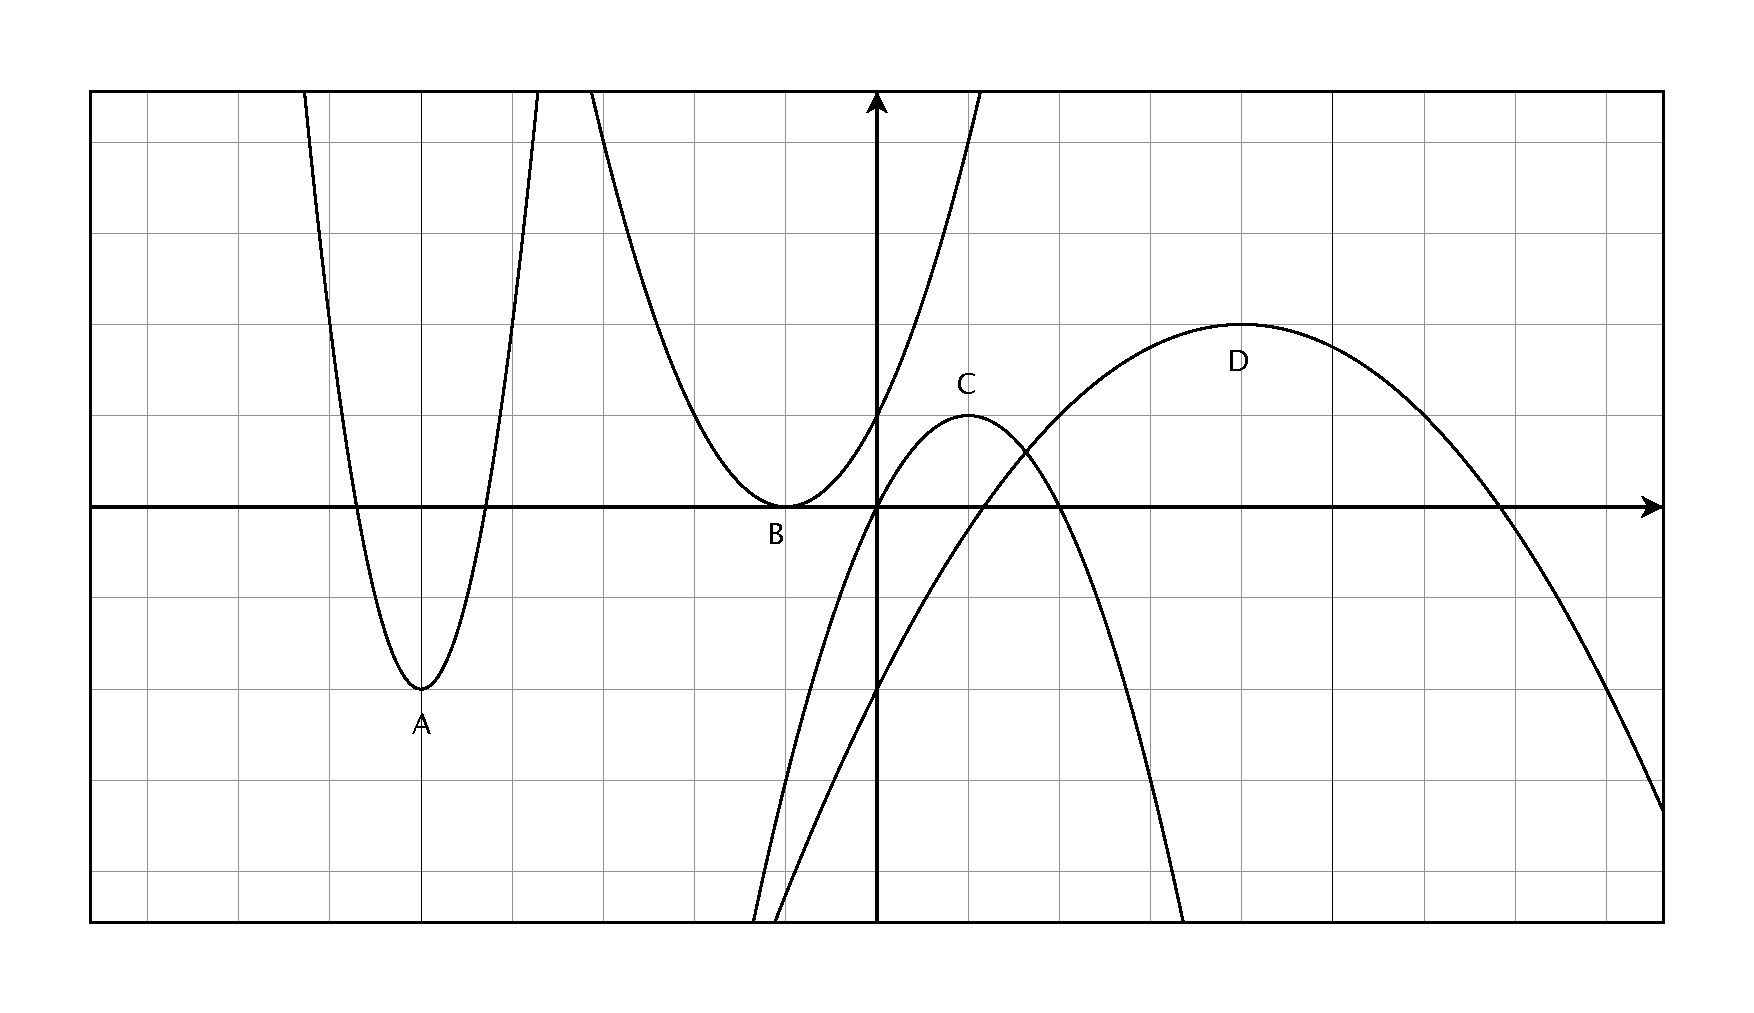
\includegraphics[scale=.3]{problem_7.eps}
%   \caption*{Problem 7}
% \end{figure}

% \begin{tabular}{cc}
% \toprule
% period & amplitude \\
% \midrule
%   $\pi$ & $2$ \\
% \bottomrule
% \end{tabular}

\title{Math 141 Notes \\ Section 3.4}
\date{April 24, 2013}

\begin{document}

  \maketitle
  \tableofcontents

  \section{Complex Numbers}

  \subsection{Definition}
  \begin{itemize}
    \item Solution to $x^2 + 1 = 0$

    \item $i = \sqrt{-1}$
      
    \item The {\em Principle Square Root} of $-r$ is $\sqrt{-r} = i \sqrt{r}$

    \item $-i \sqrt{r}$ is also a square root.

  \end{itemize}

  examples:
  \begin{align*}
    \sqrt{-3} &= 2i \\
    \sqrt{-5} &= i \sqrt{5} \\
    \sqrt{-2} \sqrt{-3} &= i \sqrt{2} \cdot i \sqrt{3} = i^2 \sqrt{6} = -6 \\
  \end{align*}

  \subsection{Real and Imaginary Parts}

  \[
    a + bi
  \]

  examples:
  \begin{align*}
    3 + 4i \\
    \frac{1}{2} + \frac{3}{4}i \\
    2 - \sqrt{2}i \\
  \end{align*}

  \subsection{Adding and Subtracting Complex Numbers}

  \begin{align*}
    (2 + 3i) + (4 - 5i) &= 6 - 2i \\
    2i - (1 + 7i) &= -1 - 5i \\
  \end{align*}

  \subsection{Multiplying Complex Numbers}
  Use FOIL.

  \subsection{Dividing Complex Numbers}

  \begin{itemize*}
    \item Define complex conjugate
    \item Bar symbol for complex conjugate
    \item Multiply by complex conjugate to simplify fractions 
  \end{itemize*}

  examples:
  \begin{itemize}
    \item $\frac{2 + 5i}{1 - i}$, etc.
    \item $\frac{2 + i}{i}$
    \item $(4 + i)^{-1}$
  \end{itemize}

  \subsection{Powers of $i$}
  \begin{align*}
    i^3 = i^2 i = -i \\
    i^4 = \left( i^2 \right)^2 = 1 \\
    i^{20} = \left( i^2 \right)^{10} = 1 \\
    i^{23} = \left( i^2 \right)^{11} i = -i \\
  \end{align*}

  \section{Complex Roots of Equations}

  \subsection{Description}
  \begin{itemize*}
    \item use quadratic equation
    \item answers always come in complex conjugate pairs
  \end{itemize*}

  \subsection{Examples}
  \begin{enumerate}
    \item 
      \begin{align*}
        f(x) &= x^2 - 2x + 2 \\
        x &= \left\{ 1 \pm i \right\} \\
      \end{align*}

    \item 
      \begin{align*}
        f(x) &= x^2 + 3 x + 5 \\
        x &= \left\{ \frac{1}{2} \left(-3 \pm i \sqrt{11}\right) \right\} \\
      \end{align*}

    \item 
      \begin{align*}
        f(x) &= -2 x^2 - x - 1 \\
        x &= \left\{ \frac{1}{4} \left(-1 \pm i \sqrt{7}\right) \right\} \\
      \end{align*}

    \item 
      \begin{align*}
        f(x) &= x - 2 + \frac{4}{x} \\
        x &= \left\{ 1 \pm i \sqrt{3} \right\} \\
      \end{align*}
  \end{enumerate}

  \section{$\sqrt{i}$}

  \begin{align*}
    (a + bi)^2       &= i \\
    a^2 + 2abi - b^2 &= i \\
    \\
    a^2 - b^2 &= 0 \\
    a         &= b \\
    \\
    2ab &= 1 \\
    a^2 &= \frac{1}{2} \\
    a   &= \frac{\sqrt{2}}{2} \\
    \\
    \sqrt{i} &= \pm \frac{\sqrt{2}}{2} \pm \frac{\sqrt{2}}{2} i \\
  \end{align*}

  Draw unit circle in complex plane, with $i^0$, $i^1$, $i^2$, $i^3$, $i^{1/2}$

  \section{Complex Conjugate Facts and Proofs}

  Problems 73-78:
  \begin{enumerate}
    \item $\left( \overline{z} \right)^2 = \overline{z^2}$

    \item $\overline{\overline{z}} = z$

    \item $z + \overline{z}$ is a real number

    \item $z - \overline{z}$ is a pure imaginary number

    \item $z \cdot \overline{z}$ is a real number
  \end{enumerate}

\end{document}

